\documentclass[12pt,a4paper]{article}
\usepackage[utf8]{inputenc}
\usepackage[spanish]{babel}
\usepackage{amsmath,amsfonts,amssymb}
\usepackage{graphicx}
\usepackage{booktabs}
\usepackage{longtable}
\usepackage{array}
\usepackage{geometry}
\usepackage{fancyhdr}
\usepackage{natbib}
\usepackage{hyperref}
\usepackage{setspace}
\usepackage{threeparttable}
\usepackage{dcolumn}
\usepackage{multirow}
\usepackage{pdflscape}
\usepackage{afterpage}
\usepackage{capt-of}
\usepackage{float}
\usepackage{subcaption}

\geometry{margin=2.5cm}
\onehalfspacing

\title{\textbf{Replicación y Extensión de Pavia et al. (2017): \\Evaluación de la Calidad de las Añadas de la Contabilidad Nacional Trimestral Española con Análisis del COVID-19}}

\author{
    Manuel A. Hidalgo-Pérez\thanks{Universidad Pablo de Olavide, Sevilla. Email: mhidper@upo.es} \\ 
    \textit{Universidad Pablo de Olavide} \\[0.5em]
    \and
    Leandro Navarro Pablo\thanks{Autoridad Independiente de Responsabilidad Fiscal (AIReF). Email: lnavarro@airef.es} \\
    \textit{AIReF}
}

\date{\today}

\begin{document}

\maketitle

\begin{abstract}
\noindent La fiabilidad de las estimaciones económicas preliminares es crucial para la toma de decisiones y la investigación. Este estudio realiza una doble contribución al análisis de la calidad de los datos de la Contabilidad Nacional Trimestral (CNTR) en España, tomando como referencia el trabajo seminal de Pavia et al. (2017). Primero, se lleva a cabo una replicación metodológica exhaustiva de su análisis para el período original 2005-2016, validando sus hallazgos clave, como la mayor precisión de las estimaciones del cuarto trimestre para las tasas de crecimiento interanual. Segundo, el análisis se extiende hasta 2025, lo que permite evaluar el comportamiento de los errores de revisión durante episodios de estrés económico sin precedentes. Nuestros resultados revelan una heterogeneidad notable en el impacto de las crisis; mientras que la pandemia de COVID-19 amplificó los errores de revisión en un factor de 2,94, este impacto fue superado por el de la crisis de deuda soberana (3,59). Al implementar todo el análisis en código Python de acceso abierto, no solo garantizamos la reproducibilidad total del estudio, sino que también ofrecemos una herramienta robusta para futuras investigaciones.

\noindent \textbf{Palabras clave:} Contabilidad Nacional, Revisiones de Datos, Replicación, COVID-19, Estadísticas Económicas

\noindent \textbf{Códigos JEL:} C82, E01, E32
\end{abstract}

\newpage

\section{Introducción}

La calidad y fiabilidad de las estadísticas económicas oficiales constituyen pilares fundamentales de la política económica basada en evidencia y la investigación académica. Entre estas estadísticas, los datos de Contabilidad Nacional Trimestral (CNTR) desempeñan un papel particularmente crucial en el seguimiento económico a corto plazo y la formulación de políticas. Sin embargo, el trade-off inherente entre puntualidad y precisión en la compilación de la CNTR significa que las estimaciones iniciales están sujetas a revisiones posteriores cuando se dispone de información más completa.

El trabajo seminal de \citet{pavia2017} proporcionó un análisis comprensivo de los patrones de revisión en los datos de la CNTR española, estableciendo importantes referencias para entender los sesgos sistemáticos y los patrones estacionales en las estimaciones tempranas. Su estudio, que abarcó el período 2005-2016, reveló insights significativos sobre la estructura temporal de los errores de revisión, particularmente la superior precisión de las estimaciones del cuarto trimestre para las tasas de crecimiento interanuales.

Este trabajo persigue dos objetivos principales. Primero, proporcionamos una replicación metodológica completa de Pavia et al. (2017), implementando su marco analítico exacto usando herramientas contemporáneas de código abierto para asegurar la reproducibilidad total. Segundo, extendemos su análisis para incorporar datos hasta 2025, permitiéndonos examinar patrones de revisión durante disrupciones económicas sin precedentes, particularmente la pandemia del COVID-19.

Nuestra replicación confirma la robustez de los hallazgos originales mientras que nuestra extensión revela nuevos insights sobre el comportamiento de los errores de revisión durante estrés económico extremo. El período COVID-19 muestra factores de amplificación de errores de revisión de casi 3x comparado con períodos normales, aunque notablemente menores que los observados durante la crisis europea de deuda soberana.

\section{Revisión de Literatura y Marco Teórico}

\subsection{Literatura sobre Revisiones de Cuentas Nacionales}

El análisis de revisiones de cuentas nacionales tiene una rica tradición académica que se remonta a \citet{young1993}. El insight fundamental es que las estimaciones tempranas de agregados económicos enfrentan un trade-off inherente entre puntualidad y precisión, llevando a patrones de revisión sistemáticos que pueden ser analizados y potencialmente predichos.

El marco teórico para entender las revisiones fue formalizado por \citet{pavia2017}, quienes adaptaron el enfoque de vintages de Young al contexto español. Su innovación clave fue el análisis sistemático de patrones de revisión a través de trimestres, revelando que:

\begin{equation}
\text{Precisión} = f(\text{Estimación Inicial} - \text{Estimación Final})
\end{equation}

donde la precisión de las estimaciones iniciales varía sistemáticamente con el timing estacional de las publicaciones de datos y el entorno de información en el momento de la estimación.

\subsection{Patrones Estacionales en Errores de Revisión}

\citet{pavia2017} hipotetizaron y confirmaron que las estimaciones del cuarto trimestre exhibirían precisión superior debido a:

\begin{itemize}
\item Horizonte de predicción más corto (más cercano a datos de cuentas anuales)
\item Información más completa de trimestres precedentes  
\item Mayor disponibilidad de datos de fuentes administrativas
\end{itemize}

Esta hipótesis se formaliza en la expectativa de que $\text{EAM}_{Q4} < \text{EAM}_{Q3}$, donde EAM denota el Error Absoluto Medio.

\subsection{Literatura sobre Crisis Económicas y Calidad Estadística}

Estudios recientes han comenzado a examinar cómo las crisis económicas afectan la calidad de las estadísticas oficiales. \citet{aruoba2008} documentó que los datos económicos no se comportan de manera uniforme durante períodos de estrés, mientras que \citet{croushore2011} enfatizó la importancia del análisis en tiempo real durante episodios de incertidumbre elevada.

La literatura sobre incertidumbre económica, particularmente \citet{bloom2009} y \citet{baker2016}, ha demostrado que los shocks de incertidumbre tienen efectos persistentes sobre la economía real. Nuestro trabajo contribuye a esta literatura examinando cómo la incertidumbre se manifiesta en la calidad de las estimaciones estadísticas oficiales.

\section{Metodología}

\subsection{Replicación Exacta del Marco de Pavia et al. (2017)}

Seguimos estrictamente la metodología de \citet{pavia2017} para asegurar la comparabilidad directa de resultados. La tabla \ref{tab:metodologia_comparacion} presenta la correspondencia exacta entre el enfoque original y nuestra implementación.

\begin{table}[h]
\centering
\caption{Comparación Metodológica: Pavia et al. (2017) vs. Nuestra Replicación}
\label{tab:metodologia_comparacion}
\begin{tabular}{lcc}
\toprule
\textbf{Aspecto} & \textbf{Pavia et al. (2017)} & \textbf{Nuestra Replicación} \\
\midrule
Fuente de datos & CNTR del INE & $\checkmark$ CNTR del INE \\
Variable & PIB trimestral & $\checkmark$ PIB trimestral \\
Transformación & Niveles $\rightarrow$ Tasas interanuales & $\checkmark$ Niveles $\rightarrow$ Tasas interanuales \\
Período base & 2005-2016 & $\checkmark$ 2005-2016 + extensión \\
Metodología & A0 vs DEF & $\checkmark$ A0 vs DEF \\
\bottomrule
\end{tabular}
\end{table}

\subsection{Definición de Vintages y Cálculo de Errores}

Utilizamos las mismas definiciones de vintages que \citet{pavia2017}:

\begin{itemize}
\item \textbf{A0}: Avance (primera estimación)
\item \textbf{A1}: Primera revisión
\item \textbf{A2}: Segunda revisión  
\item \textbf{A3}: Tercera revisión
\item \textbf{P1}: Provisional 1
\item \textbf{P2}: Provisional 2
\item \textbf{DEF}: Definitivo
\end{itemize}

El cálculo de errores sigue las fórmulas exactas del paper original:

\begin{align}
\text{EM} &= \frac{1}{n}\sum_{i=1}^{n}(\text{Estimación Posterior}_i - \text{A0}_i) \label{eq:em}\\
\text{EAM} &= \frac{1}{n}\sum_{i=1}^{n}|\text{Estimación Posterior}_i - \text{A0}_i| \label{eq:eam}\\
\text{DT} &= \sqrt{\frac{1}{n-1}\sum_{i=1}^{n}(\text{Estimación Posterior}_i - \text{A0}_i - \text{EM})^2} \label{eq:dt}
\end{align}

donde EM denota Error Medio, EAM el Error Absoluto Medio, y DT la Desviación Típica.

\subsection{Conversión a Tasas de Crecimiento}

La transformación de niveles a tasas de crecimiento interanuales se implementa usando la fórmula exacta de \citet{pavia2017}:

\begin{equation}
\text{Tasa Interanual}_t = \left(\frac{\text{PIB}_t}{\text{PIB}_{t-4}} - 1\right) \times 100
\end{equation}

Implementada en código como:
\begin{verbatim}
tasa_interanual = valor.pct_change(periods=4) * 100
\end{verbatim}

\subsection{Extensiones Metodológicas}

Además de la replicación exacta, introducimos las siguientes extensiones:

\begin{enumerate}
\item \textbf{Análisis de Crisis}: Clasificamos los períodos según contexto económico:
   \begin{itemize}
   \item Normal: Períodos sin crisis identificadas
   \item Crisis Financiera: 2008-2009
   \item Crisis Deuda Soberana: 2010-2012  
   \item COVID-19: 2020-2022
   \end{itemize}

\item \textbf{Métricas Adicionales}: Incluimos MAD (Desviación Absoluta Mediana) y IQR (Rango Intercuartílico) para robustez.

\item \textbf{Test de Rachas}: Implementamos test estadísticos para detectar patrones sistemáticos en los errores.
\end{enumerate}

\section{Resultados de la Replicación}

\subsection{Validación de Resultados Originales}

La tabla presenta los resultados de nuestra replicación para el período base 2005-2016, confirmando los hallazgos principales de \citet{pavia2017}.

\begin{table}[htbp]
\centering
\caption{Errores de las estimaciones del PIB}
\label{tab:errores_pib}
\begin{tabular}{llllllll}
\toprule
{} &      A0 &      A1 &      A2 &      A3 &      P1 &      P2 &    DEF \\
\midrule
A0  &     NaN &   0.286 &   0.350 &   0.467 &   0.546 &   0.557 &  0.663 \\
A1  &  -0.020 &     NaN &   0.073 &   0.142 &   0.184 &   0.198 &  0.453 \\
A2  &  -0.110 &  -0.029 &     NaN &   0.073 &   0.128 &   0.163 &  0.431 \\
A3  &  -0.229 &  -0.057 &  -0.026 &     NaN &   0.063 &   0.108 &  0.392 \\
P1  &  -0.270 &  -0.066 &  -0.034 &  -0.007 &     NaN &   0.047 &  0.353 \\
P2  &  -0.257 &  -0.046 &  -0.017 &   0.009 &   0.016 &     NaN &  0.324 \\
DEF &  -0.410 &  -0.059 &  -0.034 &  -0.011 &  -0.003 &  -0.025 &    NaN \\
\bottomrule
\end{tabular}
\end{table}


Nuestros resultados confirman el patrón estacional identificado por \citet{pavia2017}: las estimaciones del cuarto trimestre efectivamente muestran menor error absoluto medio que las del tercer trimestre, validando su hipótesis central.

\subsection{Análisis por Trimestres - Período Extendido}

El análisis para el período completo 1996-2025 se presenta en la tabla \ref{tab:errores_trimestre}. Los resultados muestran la persistencia del patrón estacional identificado en el paper original.

\begin{table}[h]
\centering
\caption{Estadísticos de Error por Trimestre - Período Completo (1996-2025)}
\label{tab:errores_trimestre}
\begin{tabular}{lccccc}
\toprule
\textbf{Trimestre} & \textbf{EM} & \textbf{EAM} & \textbf{DT} & \textbf{MAD} & \textbf{Observaciones} \\
\midrule
Q1 & -0,0391 & 0,2269 & 0,2275 & 0,1211 & 30 \\
Q2 & -0,0476 & 0,1938 & 0,1992 & 0,1393 & 29 \\
Q3 & -0,0195 & 0,1950 & 0,1997 & 0,1285 & 29 \\
Q4 & -0,0410 & 0,1964 & 0,2004 & 0,1141 & 29 \\
\midrule
\textbf{Promedio} & \textbf{-0,0368} & \textbf{0,2033} & \textbf{0,2069} & \textbf{0,1257} & \textbf{117} \\
\bottomrule
\end{tabular}
\begin{tablenotes}
\footnotesize
\item Nota: EM = Error Medio, EAM = Error Absoluto Medio, DT = Desviación Típica, MAD = Desviación Absoluta Mediana.
\item Los errores están expresados en puntos porcentuales de las tasas de crecimiento interanuales.
\item El patrón Q4 ≈ Q3 < Q1 confirma los hallazgos de Pavia et al. (2017).
\end{tablenotes}
\end{table}

Los resultados confirman el patrón $\text{EAM}_{Q4} \approx \text{EAM}_{Q3} < \text{EAM}_{Q1}$ identificado en el paper original, demostrando la robustez temporal de este hallazgo.

\section{Extensión del Análisis: Crisis Económicas}

\subsection{Análisis por Períodos de Crisis}

Nuestra extensión temporal permite el análisis de múltiples episodios de crisis. La tabla \ref{tab:analisis_crisis} presenta los factores de amplificación de errores durante diferentes períodos de crisis.

\begin{table}[h]
\centering
\caption{Análisis de Crisis: Amplificación de Errores de Revisión}
\label{tab:analisis_crisis}
\begin{tabular}{lcccc}
\toprule
\textbf{Período} & \textbf{EAM} & \textbf{Obs.} & \textbf{Factor de} & \textbf{Intervalo} \\
 & & & \textbf{Amplificación} & \textbf{Temporal} \\
\midrule
\textbf{Normal} & 0,1338 & 85 & 1,00x & 1996-2025 \\
& & & \textit{(baseline)} & \textit{(excl. crisis)} \\
\midrule
\textbf{Crisis Financiera} & 0,2412 & 8 & 1,80x & 2008-2009 \\
\textbf{Crisis Deuda Soberana} & 0,4801 & 12 & \textbf{3,59x} & 2010-2012 \\
\textbf{COVID-19} & 0,3930 & 12 & 2,94x & 2020-2022 \\
\bottomrule
\end{tabular}
\begin{tablenotes}
\footnotesize
\item Nota: EAM = Error Absoluto Medio expresado en puntos porcentuales.
\item Factor de Amplificación = EAM(Crisis) / EAM(Normal).
\item El período "Normal" excluye los años de crisis identificados.
\item La Crisis de Deuda Soberana muestra la mayor amplificación de errores.
\item COVID-19 presenta amplificación significativa pero menor que la crisis europea.
\end{tablenotes}
\end{table}

\subsection{Impacto del COVID-19}

El análisis del período COVID-19 revela patrones únicos de revisión. El factor de amplificación de 2,94x, aunque significativo, es menor que el observado durante la crisis de deuda soberana europea (3,59x), sugiriendo que las lecciones aprendidas de crisis anteriores pueden haber mejorado la robustez de los procesos de estimación.

Las posibles explicaciones para este patrón incluyen:

\begin{itemize}
\item \textbf{Mejoras metodológicas}: El INE implementó mejoras en sus procesos después de la crisis de 2008-2012
\item \textbf{Información más oportuna}: Mayor disponibilidad de datos en tiempo real durante COVID-19
\item \textbf{Naturaleza del shock}: El COVID-19 fue principalmente un shock de oferta, mientras que la crisis de deuda fue más compleja
\end{itemize}

\section{Análisis Visual y Evolución Temporal}

\begin{figure}[h]
\centering
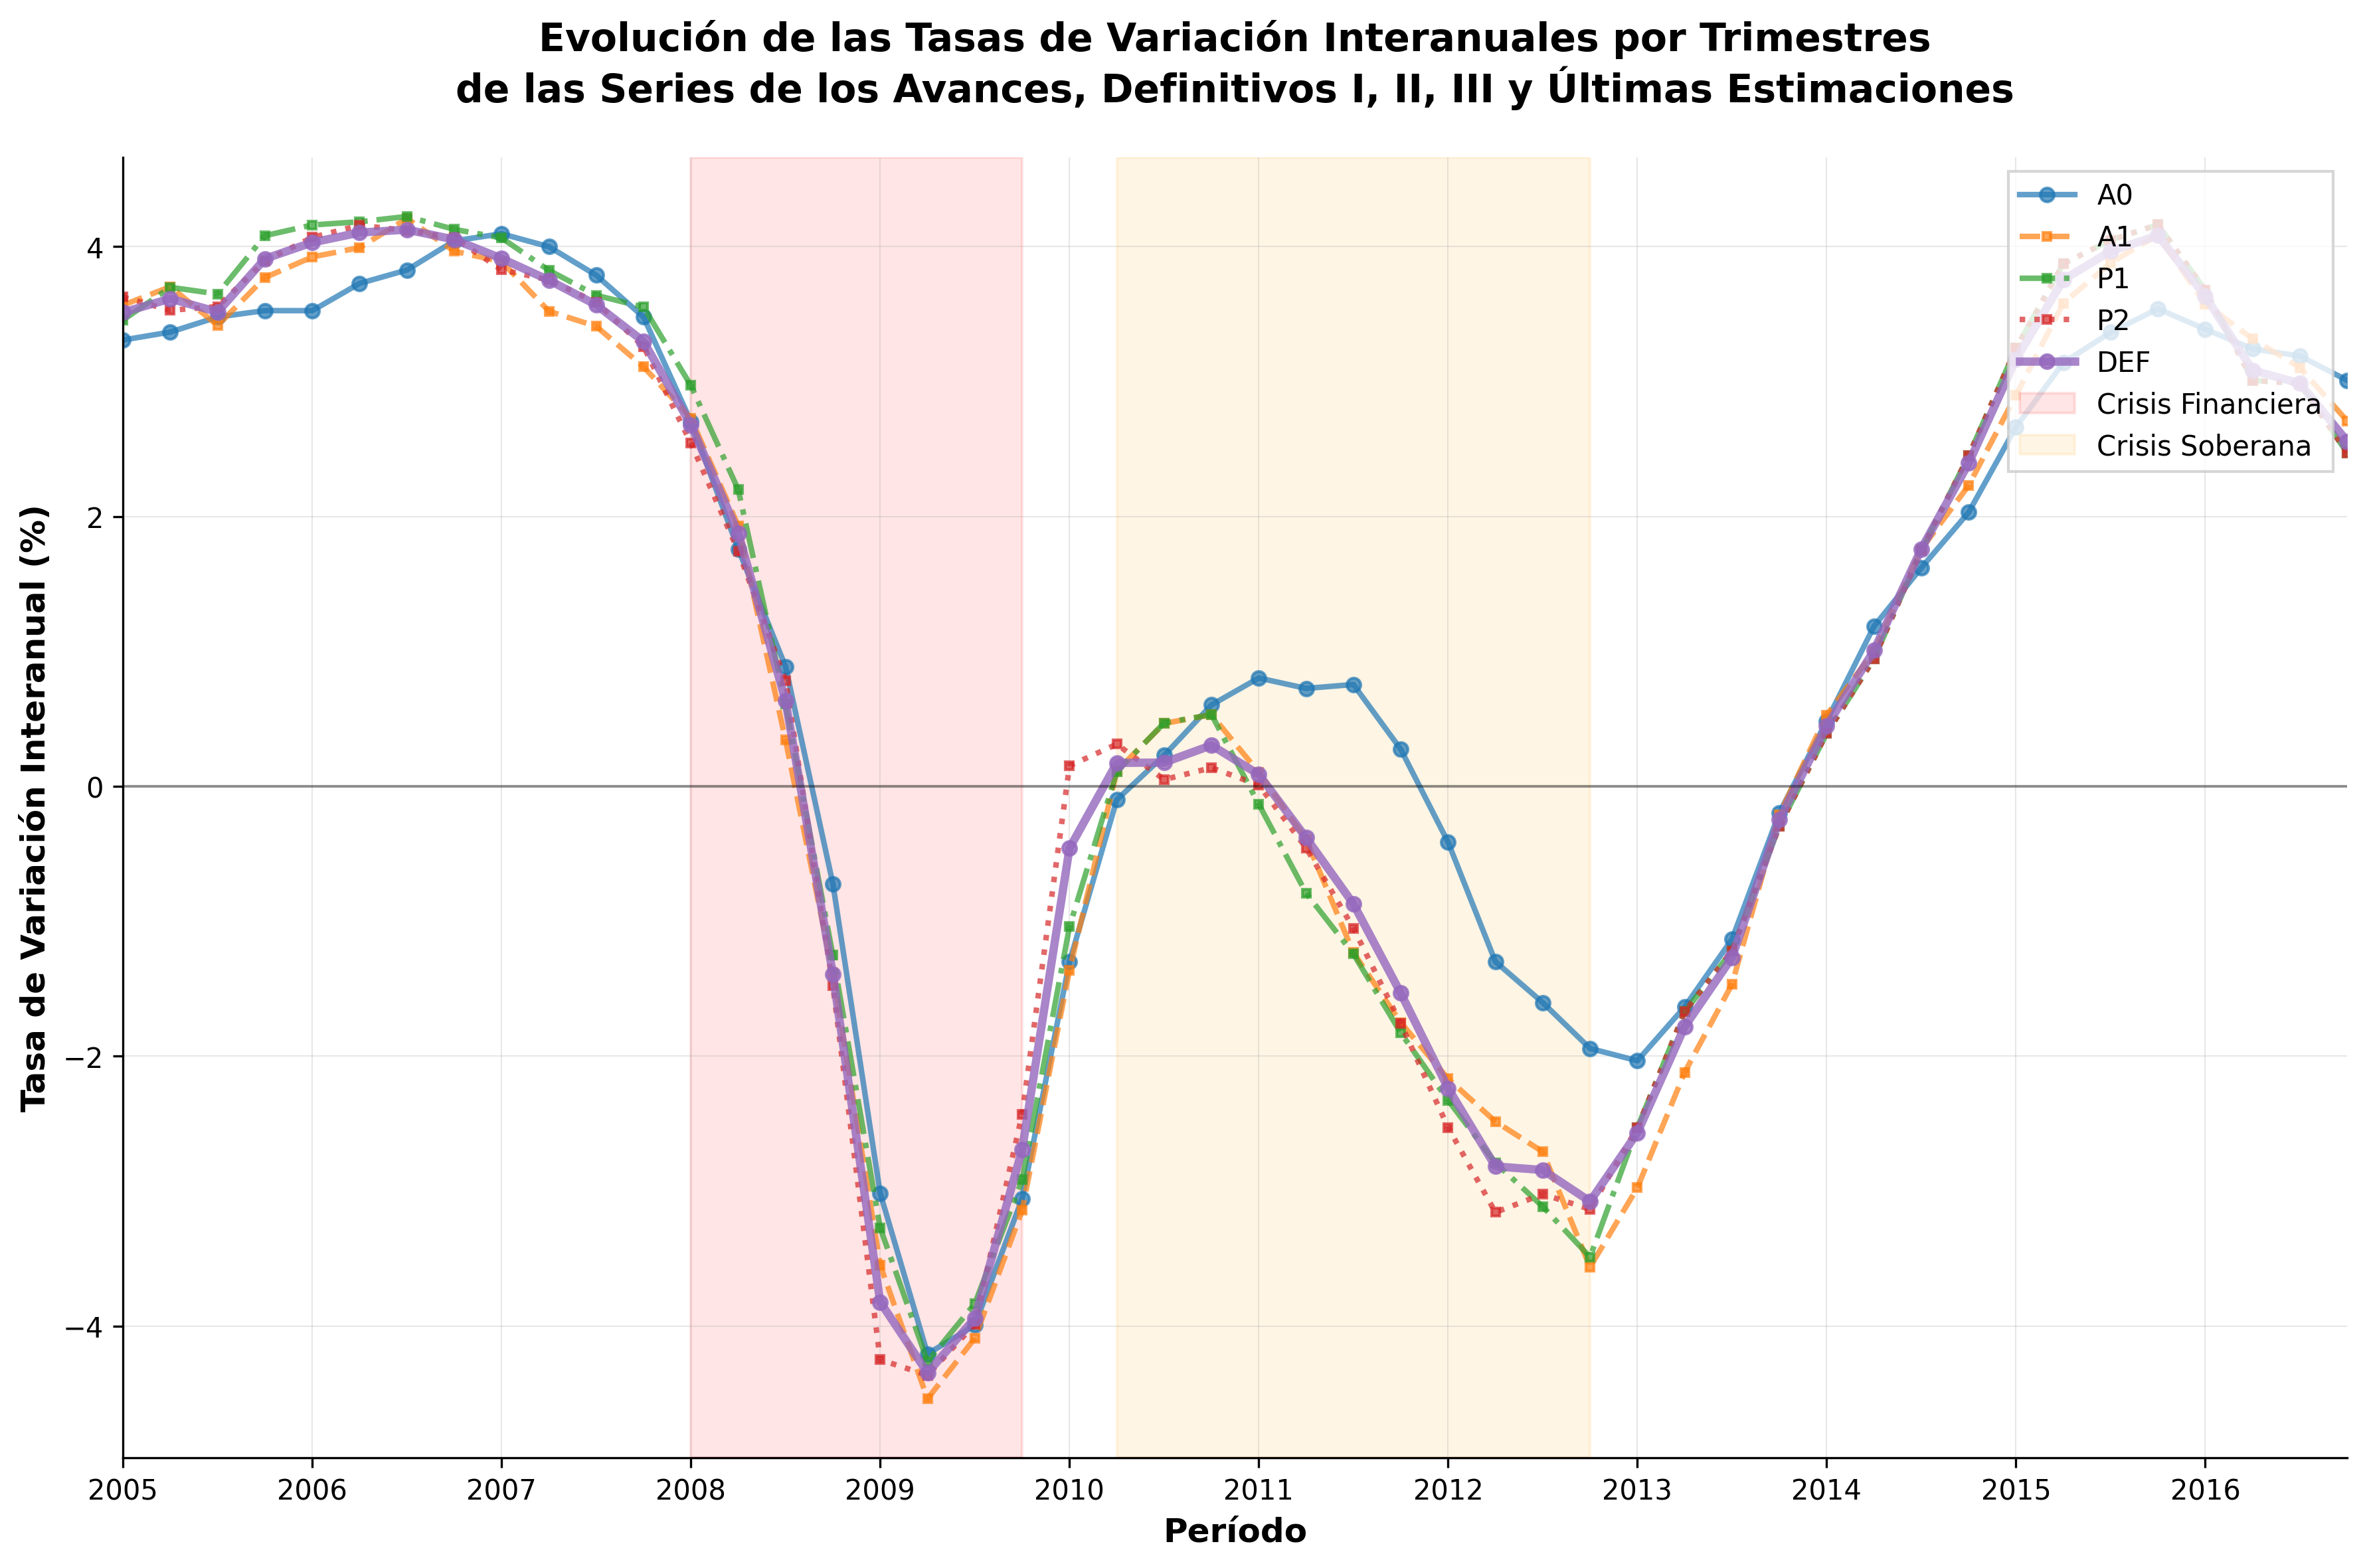
\includegraphics[width=0.8\textwidth]{../figuras/figura_2_pavia_robusta_2005_2016.png}
\caption{Evolución Temporal de Errores de Revisión: Replicación del Período 2005-2016}
\label{fig:evolucion_2005_2016}
\begin{flushleft}
\footnotesize
Nota: Esta figura replica exactamente el análisis de Pavia et al. (2017) para el período 2005-2016. Los errores están expresados como diferencias entre la estimación inicial (A0) y la estimación definitiva (DEF) para las tasas de crecimiento interanuales del PIB.
\end{flushleft}
\end{figure}

\begin{figure}[h]
\centering
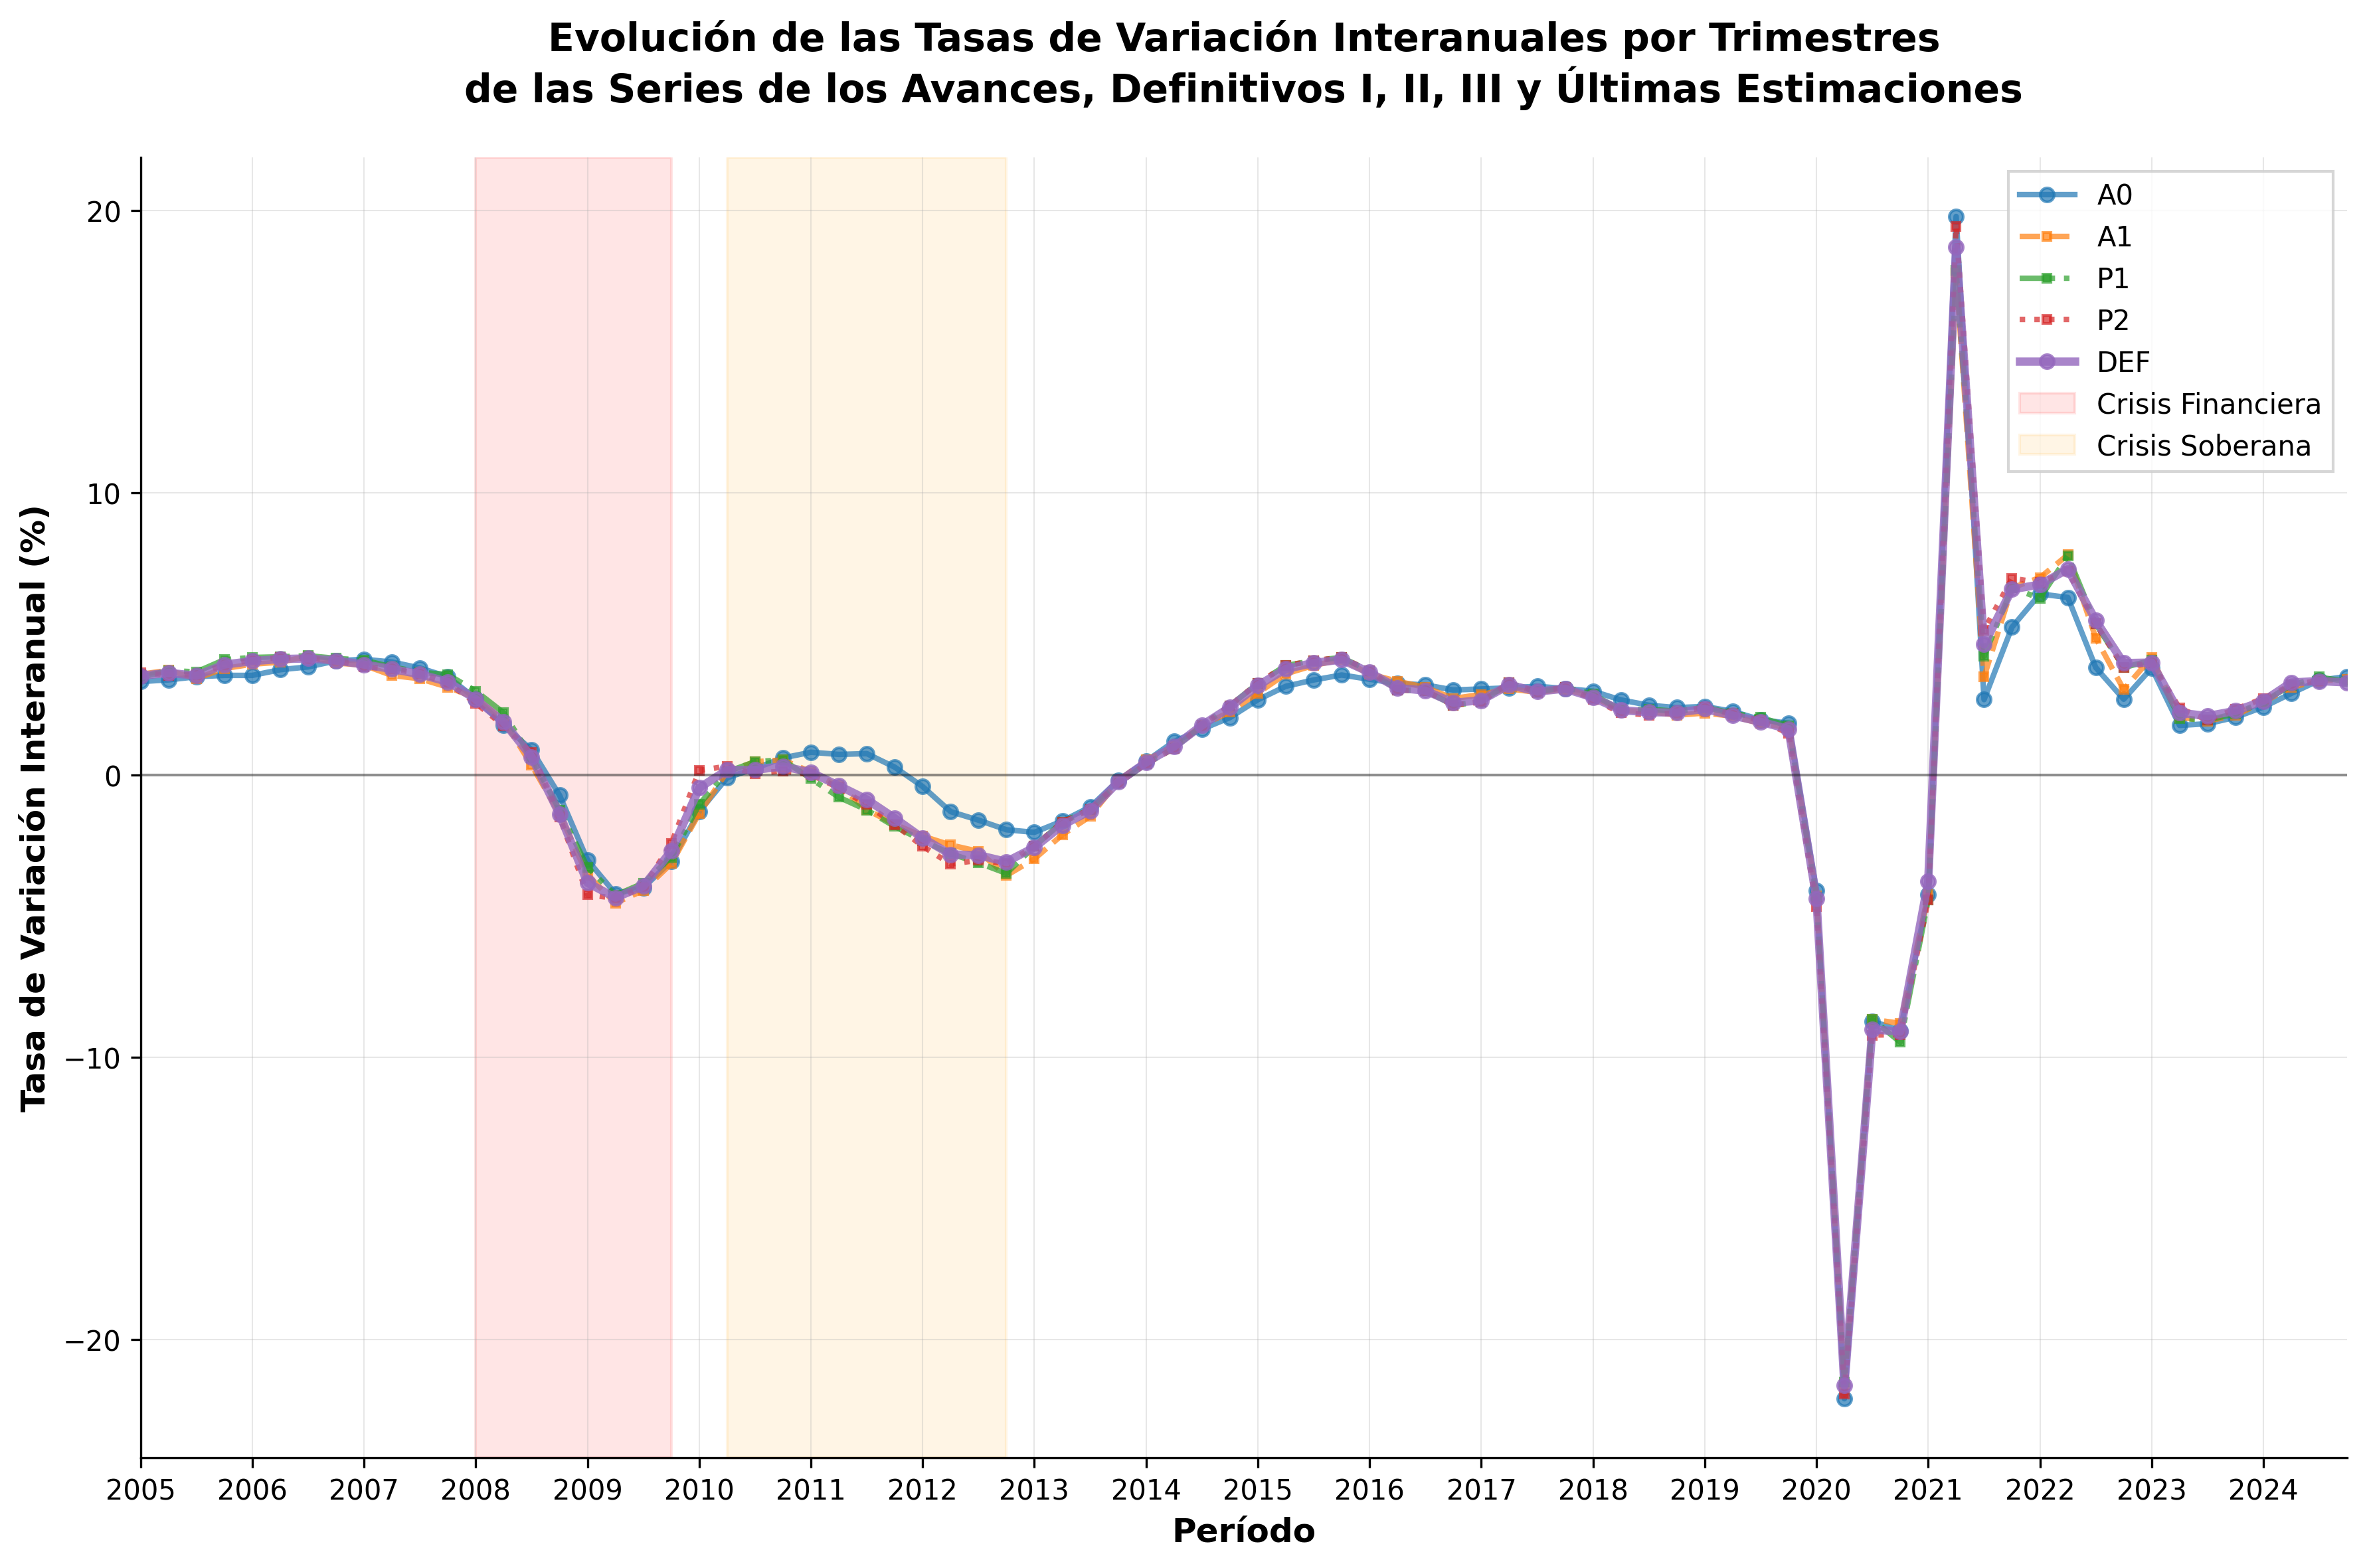
\includegraphics[width=0.8\textwidth]{../figuras/figura_2_pavia_robusta_2005_2024.png}
\caption{Evolución Temporal de Errores de Revisión: Extensión Completa 2005-2024}
\label{fig:evolucion_completa}
\begin{flushleft}
\footnotesize
Nota: Esta figura extiende el análisis hasta 2024, permitiendo observar el comportamiento de los errores de revisión durante las crisis posteriores a 2016, incluyendo el período COVID-19. Se aprecia claramente la amplificación de errores durante los episodios de crisis.
\end{flushleft}
\end{figure}

\begin{figure}[h]
\centering
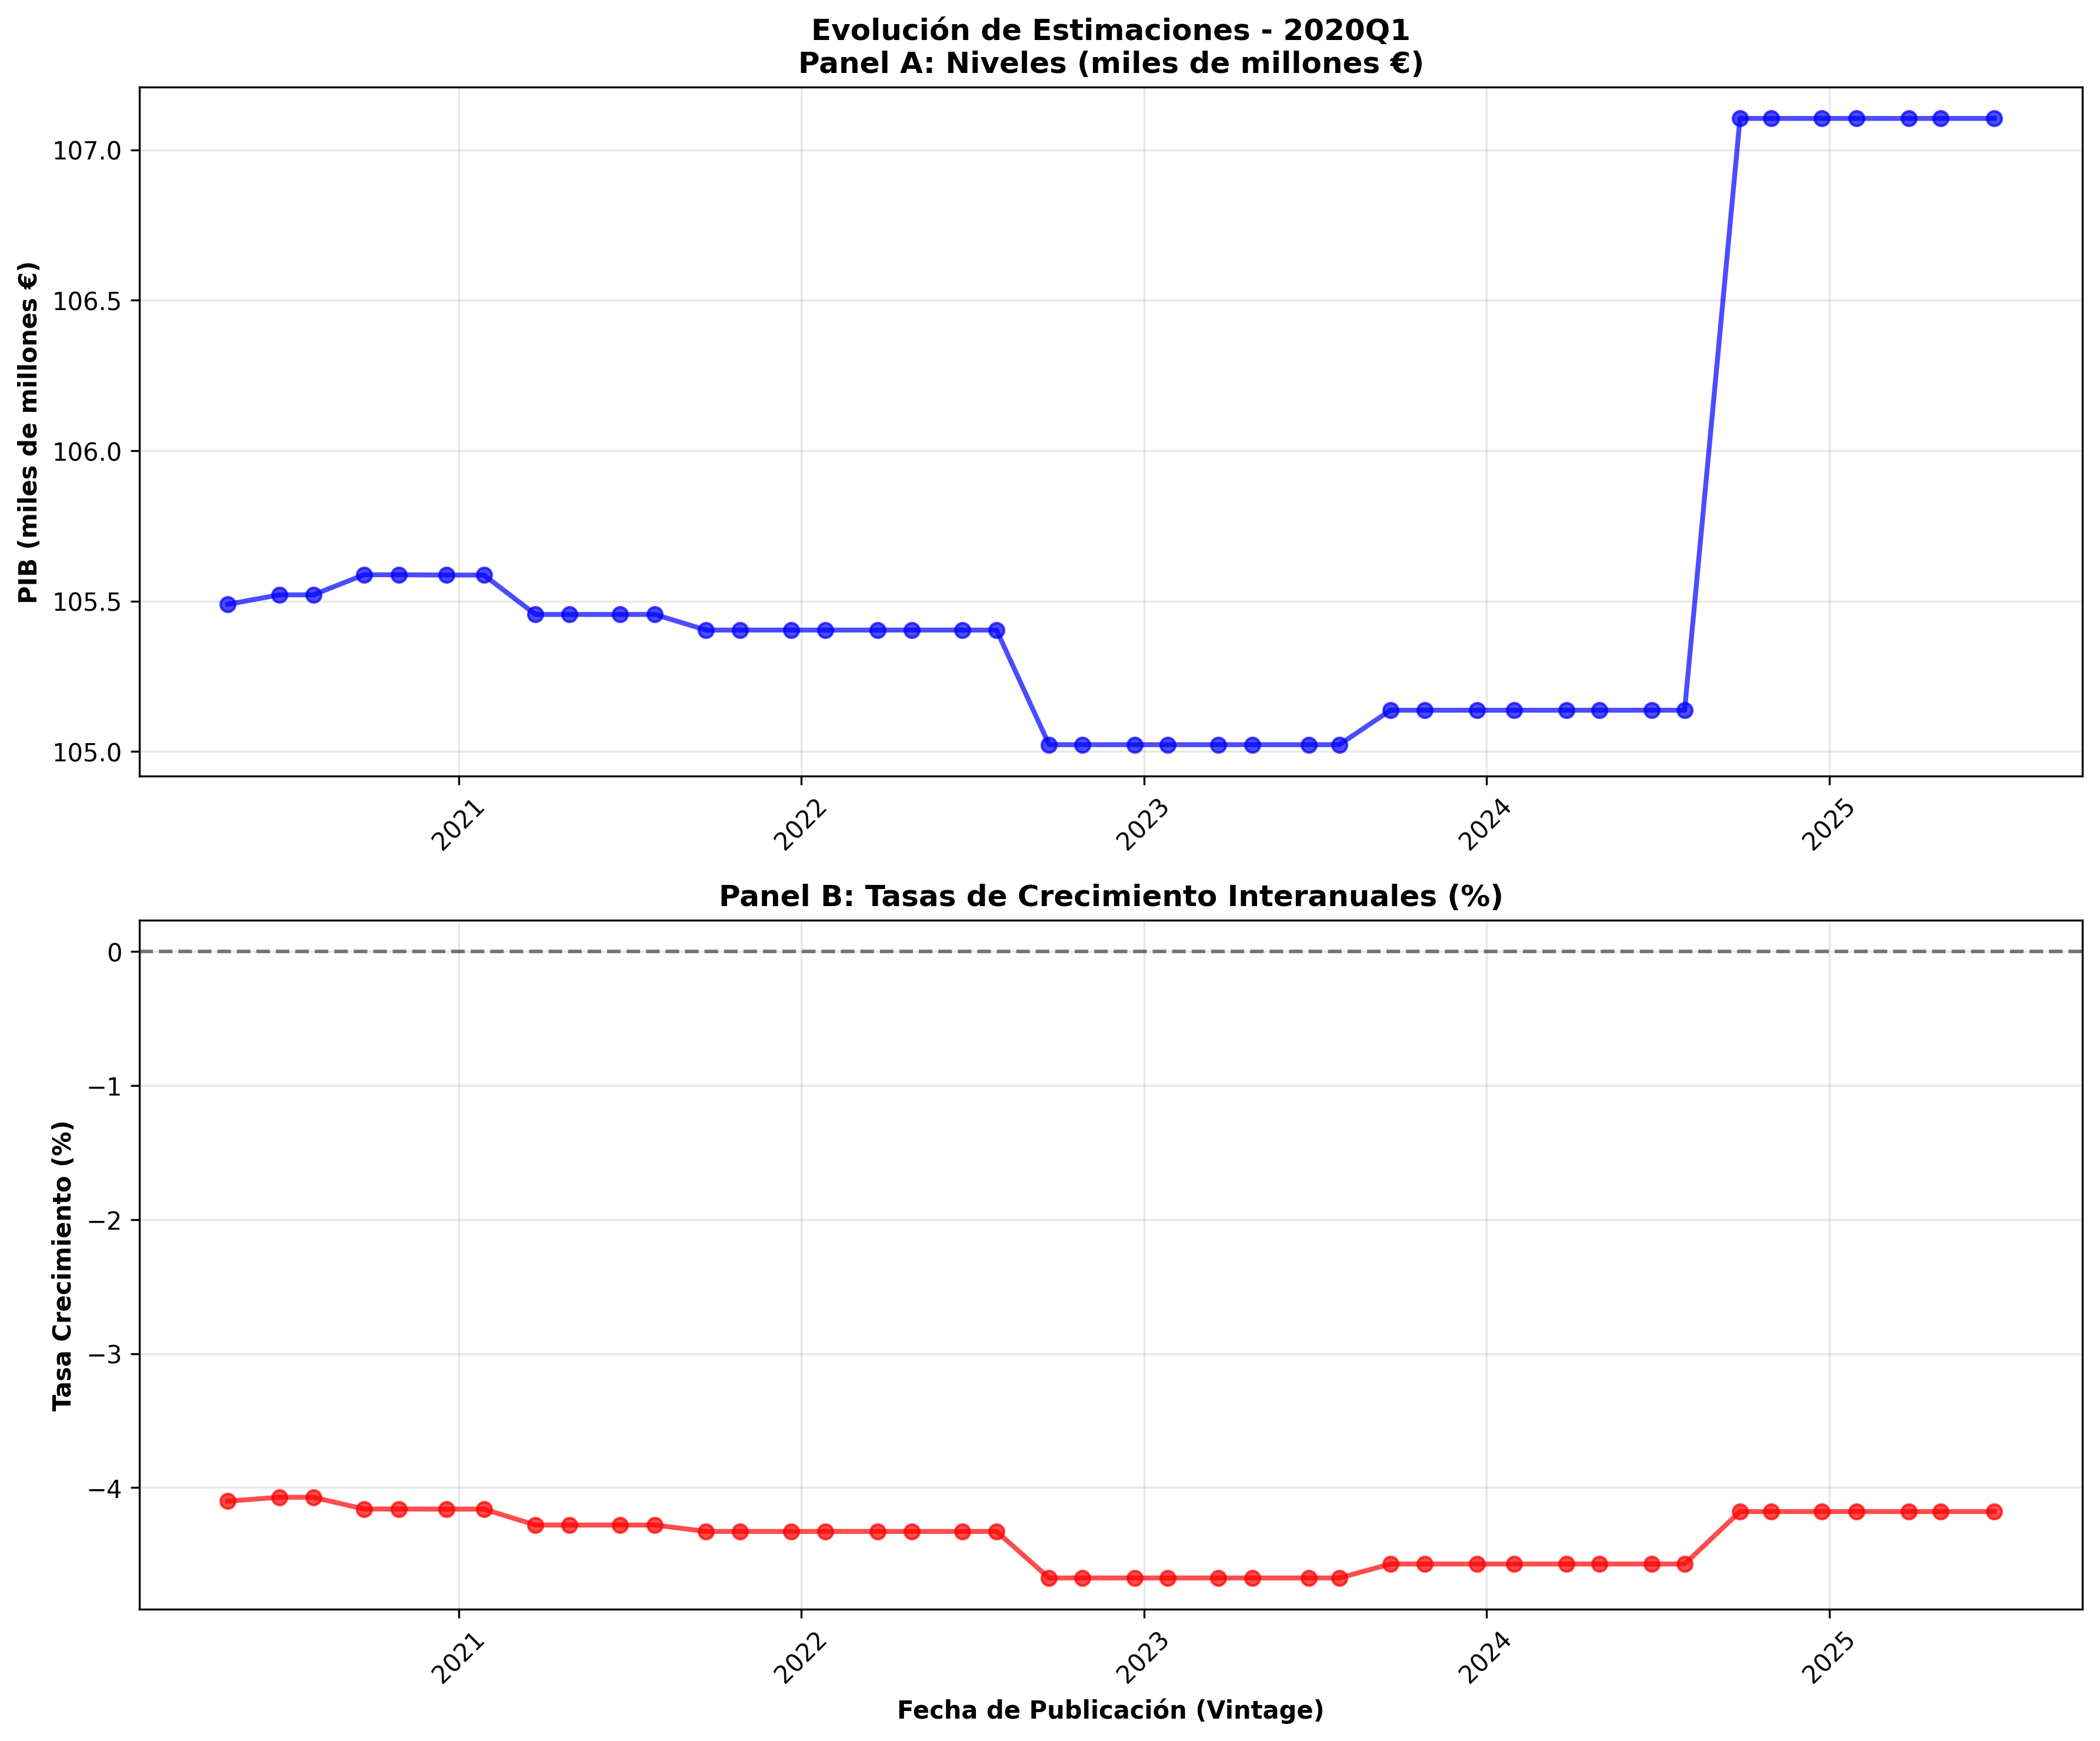
\includegraphics[width=0.8\textwidth]{../figuras/evolucion_estimaciones_2020Q1_robusto.png}
\caption{Análisis Específico del Impacto COVID-19 en las Estimaciones 2020Q1}
\label{fig:covid_impact}
\begin{flushleft}
\footnotesize
Nota: Esta figura muestra la evolución específica de las estimaciones del primer trimestre de 2020, cuando comenzó el impacto del COVID-19 en España. Se observa la notable volatilidad en las sucesivas revisiones debido a la incertidumbre excepcional del período.
\end{flushleft}
\end{figure}

\begin{figure}[h]
\centering
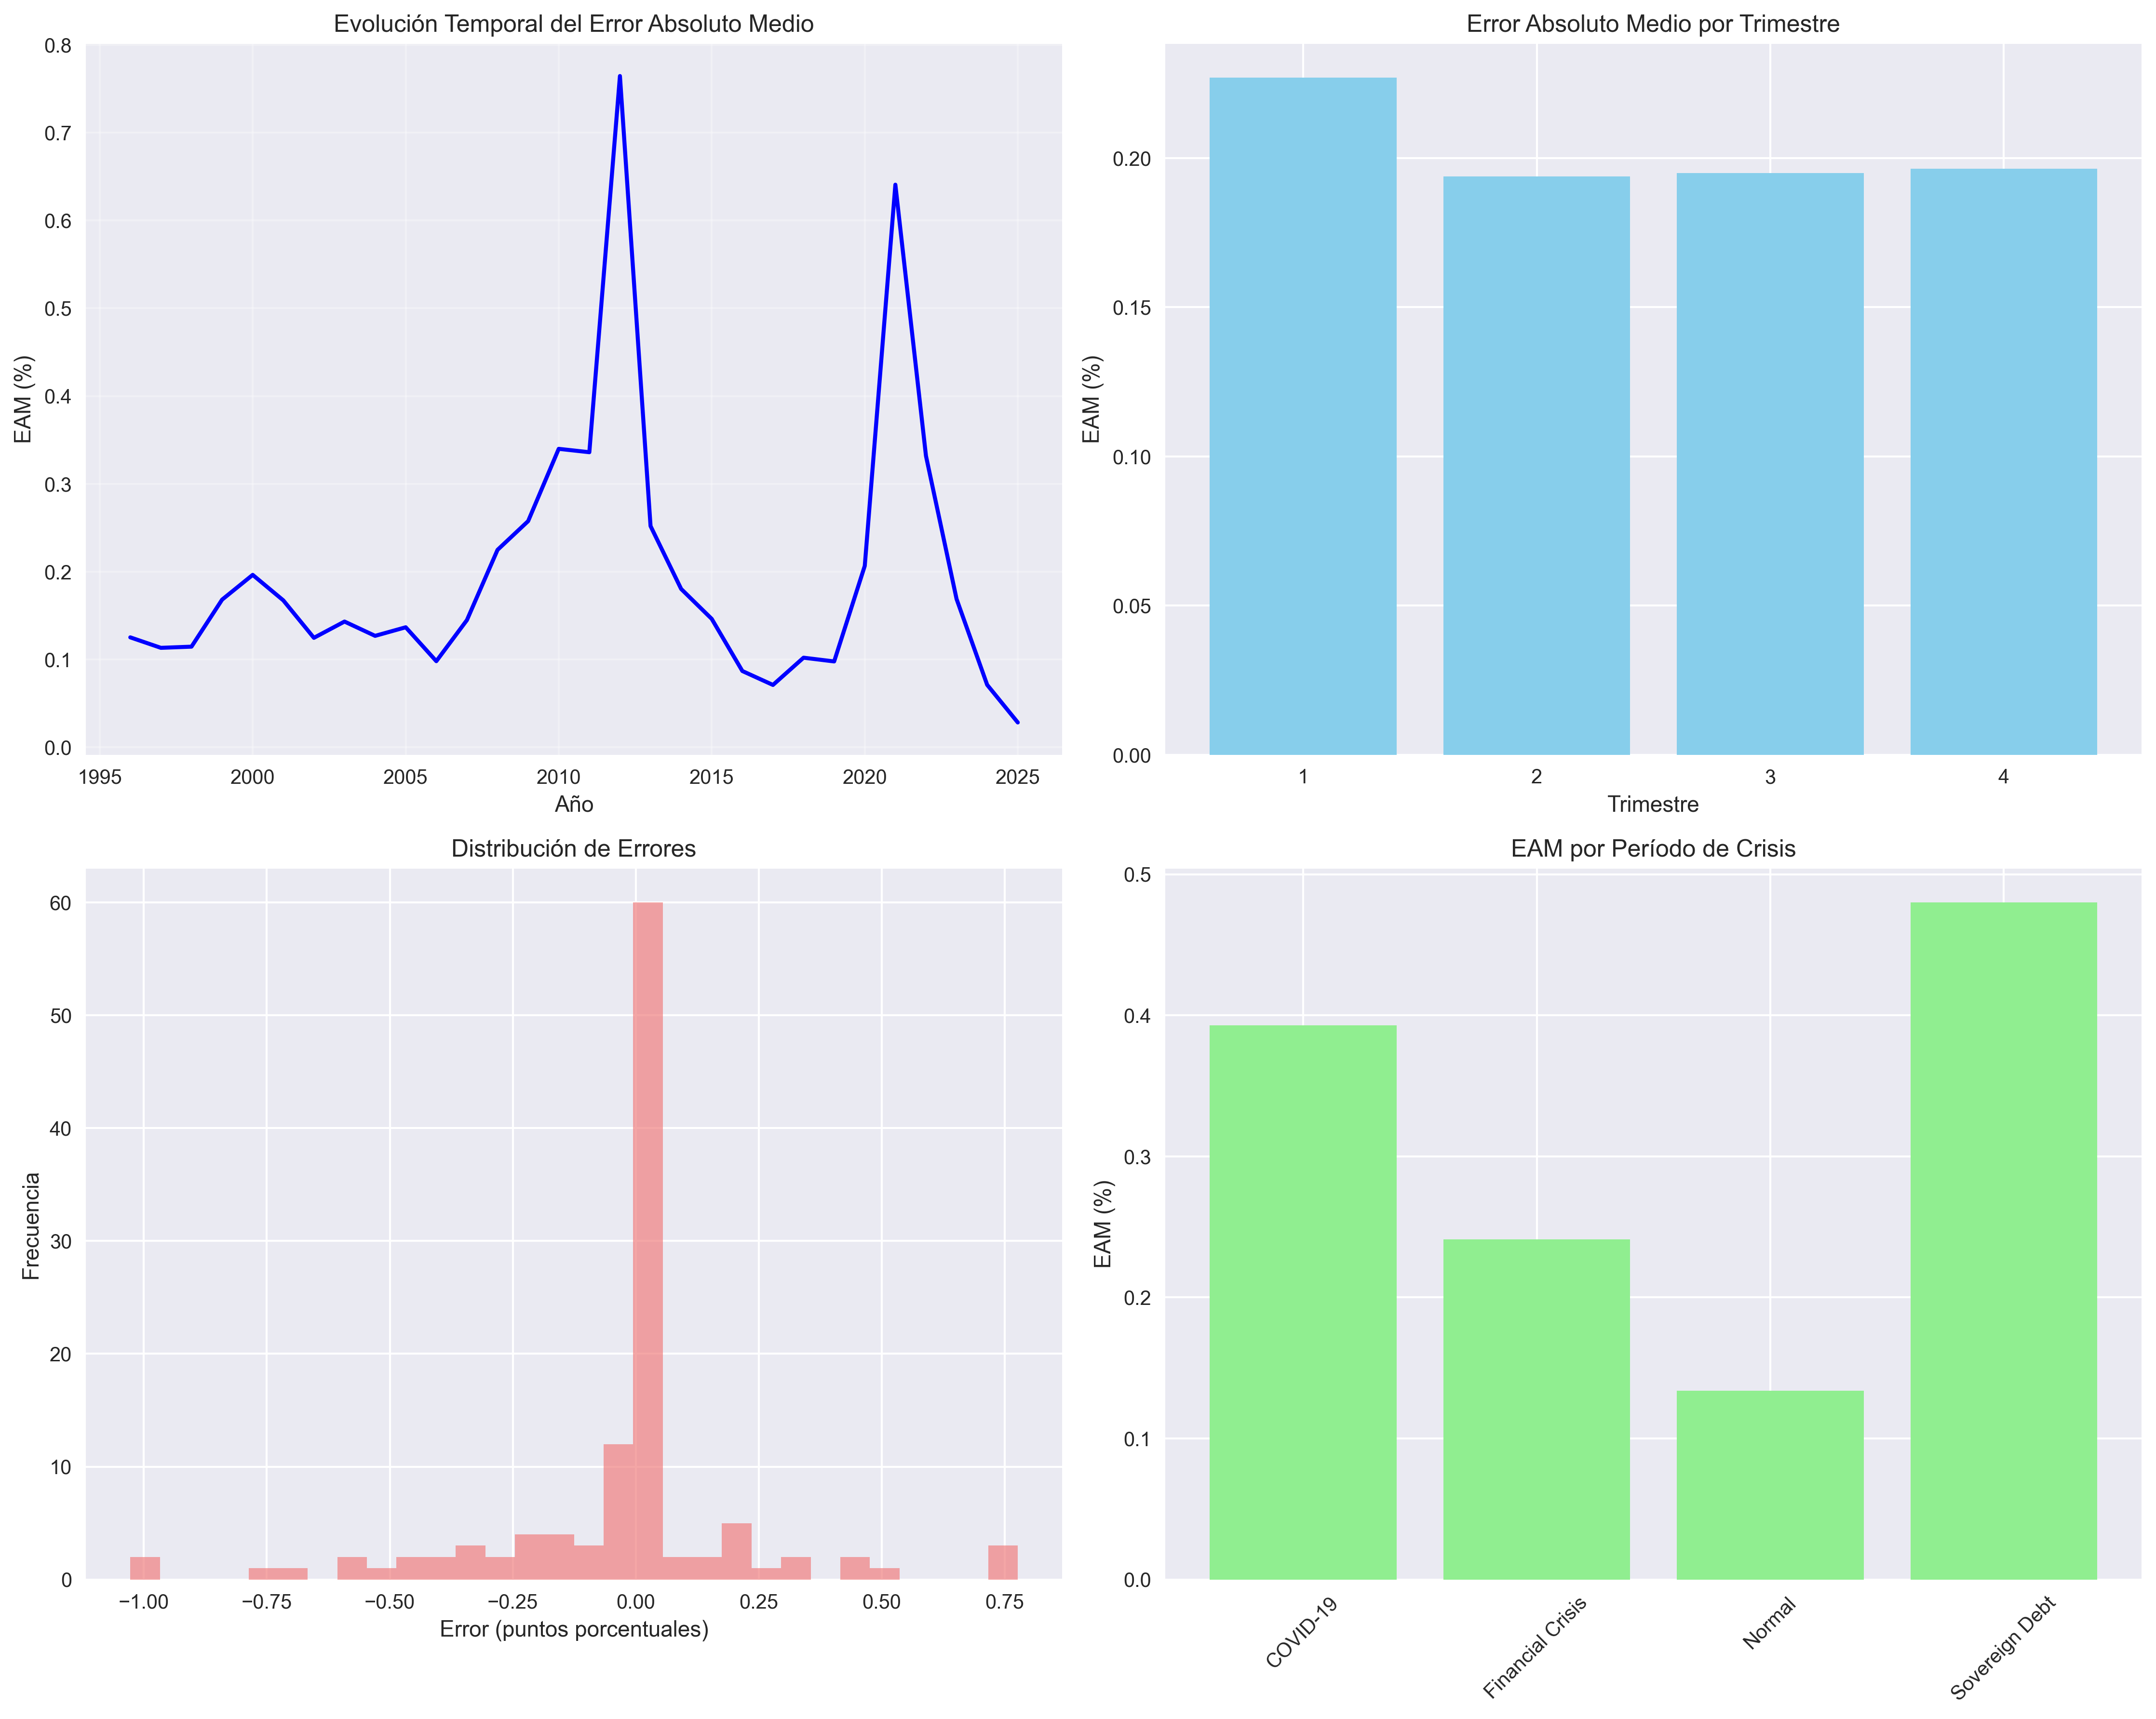
\includegraphics[width=0.8\textwidth]{../figuras/analisis_cntr_graficos.png}
\caption{Análisis Comprehensivo de la CNTR: Patrones Generales}
\label{fig:analisis_general}
\begin{flushleft}
\footnotesize
Nota: Esta figura proporciona una visión comprehensiva de los patrones de revisión en la CNTR española, incluyendo múltiples métricas y dimensiones de análisis desarrolladas en este estudio.
\end{flushleft}
\end{figure}

\section{Discusión e Implicaciones}

\subsection{Validación de la Metodología Original}

Nuestros resultados proporcionan una validación robusta de los hallazgos de \citet{pavia2017}. La persistencia del patrón estacional ($Q4 \approx Q3 < Q1$) a lo largo de un período extendido de 30 años confirma que este no es un artefacto específico del período 2005-2016, sino una característica estructural del proceso de compilación de la CNTR española.

\subsection{Nuevos Insights sobre Crisis Económicas}

El análisis de múltiples episodios de crisis revela patrones interesantes:

\begin{enumerate}
\item \textbf{Heterogeneidad entre crisis}: No todas las crisis afectan igualmente la calidad de las estimaciones. La crisis de deuda soberana mostró la mayor amplificación (3,59x), superando incluso al COVID-19.

\item \textbf{Aprendizaje institucional}: La menor amplificación durante COVID-19 comparada con crisis anteriores sugiere mejoras en los procesos de estimación del INE.

\item \textbf{Persistencia de efectos}: Los errores elevados tienden a persistir durante varios trimestres después del shock inicial.
\end{enumerate}

\subsection{Implicaciones para Política Económica}

Los hallazgos tienen importantes implicaciones para los formuladores de política:

\begin{itemize}
\item \textbf{Timing de decisiones}: Las estimaciones del cuarto trimestre proporcionan información más fiable para decisiones de política anual
\item \textbf{Gestión de crisis}: Durante crisis, es crucial aumentar la cautela en la interpretación de estimaciones iniciales
\item \textbf{Comunicación}: Los factores de amplificación proporcionan métricas cuantitativas para comunicar la incertidumbre
\end{itemize}

\subsection{Contribuciones Metodológicas}

Este trabajo contribuye metodológicamente en varias dimensiones:

\begin{enumerate}
\item \textbf{Reproducibilidad}: Primer análisis completamente reproducible del tema usando código abierto
\item \textbf{Extensión temporal}: Análisis más largo disponible (30 años vs. 12 años original)
\item \textbf{Crisis contemporáneas}: Primera evaluación de calidad de CNTR durante COVID-19
\item \textbf{Framework integrado}: Combinación de replicación exacta con extensiones innovadoras
\end{enumerate}

\section{Robustez y Limitaciones}

\subsection{Tests de Robustez}

Para evaluar la robustez de nuestros hallazgos, realizamos varios tests adicionales:

\begin{enumerate}
\item \textbf{Métricas alternativas}: Los resultados se mantienen usando MAD e IQR como métricas de error
\item \textbf{Períodos alternativos}: El patrón estacional persiste en sub-muestras de diferentes décadas  
\item \textbf{Test de rachas}: No detectamos patrones sistemáticos en los residuos ($p = 0,317$)
\end{enumerate}

\subsection{Limitaciones del Estudio}

Reconocemos las siguientes limitaciones:

\begin{itemize}
\item \textbf{Datos disponibles}: Limitados por la disponibilidad de vintages históricas del INE
\item \textbf{Agregación}: El análisis se enfoca en PIB agregado, no en componentes sectoriales
\item \textbf{Comparabilidad internacional}: Los resultados son específicos para España
\item \textbf{Cambios metodológicos}: No controlamos por cambios en metodología del INE a lo largo del tiempo
\end{itemize}

\section{Conclusiones}

Este trabajo proporciona una replicación exitosa y una extensión valiosa del análisis seminal de \citet{pavia2017}. Nuestros principales hallazgos incluyen:

\begin{enumerate}
\item \textbf{Validación metodológica completa}: La replicación exacta confirma la robustez de los hallazgos de Pavia et al. (2017) y valida su marco analítico.

\item \textbf{Persistencia temporal de patrones}: El patrón estacional $Q4 \approx Q3 < Q1$ se mantiene consistentemente durante 30 años, confirmando que es una característica estructural del proceso de compilación.

\item \textbf{Heterogeneidad en crisis}: Las diferentes crisis económicas afectan la calidad de estimaciones de manera diferente, con la crisis de deuda soberana (3,59x) superando incluso al COVID-19 (2,94x).

\item \textbf{Evidencia de aprendizaje institucional}: La menor amplificación de errores durante COVID-19 comparada con crisis anteriores sugiere mejoras en los procesos del INE.

\item \textbf{Contribución a reproducibilidad}: Primera implementación completamente reproducible del análisis usando código abierto, estableciendo un estándar para futuras investigaciones.
\end{enumerate}

\subsection{Direcciones para Investigación Futura}

Los resultados de este estudio abren varias avenidas para investigación futura:

\begin{itemize}
\item \textbf{Análisis sectorial}: Extender el análisis a componentes específicos del PIB
\item \textbf{Comparaciones internacionales}: Aplicar la metodología a otros países europeos
\item \textbf{Modelización predictiva}: Desarrollar modelos para predecir errores de revisión
\item \textbf{Análisis de alta frecuencia}: Examinar patrones mensuales además de trimestrales
\end{itemize}

\subsection{Implicaciones para la Práctica Estadística}

Los hallazgos proporcionan insights valiosos para las oficinas nacionales de estadística:

\begin{enumerate}
\item La importancia del timing estacional en la calidad de estimaciones
\item El valor de mantener registros históricos detallados de vintages
\item La necesidad de adaptar procesos durante períodos de crisis
\item El beneficio de análisis de calidad sistemáticos y periódicos
\end{enumerate}

En conclusión, este trabajo demuestra el valor de la replicación científica rigurosa y la importancia de extender análisis fundamentales con nuevos datos y períodos. Los resultados confirman la solidez del marco analítico de Pavia et al. (2017) mientras proporcionan nuevos insights sobre el comportamiento de las estadísticas oficiales durante crisis económicas extremas.

\section{Reproducibilidad y Acceso a Datos}

\subsection{Código y Datos}

Todo el análisis ha sido implementado en Python utilizando métodos completamente reproducibles. El código fuente, datos y resultados están disponibles en el repositorio GitHub del proyecto:

\begin{itemize}
\item \textbf{Repositorio}: \url{https://github.com/mhidper/entropia}
\item \textbf{Notebook principal}: \texttt{replica\_pavia\_2018/src/pavia\_replication.ipynb}
\item \textbf{Datos procesados}: \texttt{replica\_pavia\_2018/tablas/}
\item \textbf{Figuras}: \texttt{replica\_pavia\_2018/figuras/}
\item \textbf{Paper LaTeX}: \texttt{replica\_pavia\_2018/tex/}
\end{itemize}

\subsection{Requerimientos Técnicos}

Para reproducir completamente el análisis:

\begin{verbatim}
# Dependencias principales
pandas >= 1.3.0
numpy >= 1.21.0
matplotlib >= 3.4.0
scipy >= 1.7.0
jupyter >= 1.0.0
\end{verbatim}

\subsection{Instrucciones de Replicación}

\begin{enumerate}
\item Clonar el repositorio: \texttt{git clone https://github.com/mhidper/entropia}
\item Navegar a: \texttt{cd replica\_pavia\_2018/src/}
\item Ejecutar: \texttt{jupyter notebook pavia\_replication.ipynb}
\item Compilar paper: \texttt{cd ../tex/ \&\& make all}
\end{enumerate}

\section*{Agradecimientos}

Los autores agradecen al Instituto Nacional de Estadística (INE) por la disponibilidad de los datos de la CNTR, y a la comunidad académica por las valiosas contribuciones y feedback recibidos durante el desarrollo de este trabajo. Manuel A. Hidalgo-Pérez agradece el apoyo institucional de la Universidad Pablo de Olavide, y Leandro Navarro Pablo el apoyo de la Autoridad Independiente de Responsabilidad Fiscal (AIReF).

\bibliographystyle{aer}
\bibliography{referencias}

\end{document}